\documentclass[a4paper,man,natbib,floatsintext]{apa6}

\usepackage[english]{babel}
\usepackage[utf8x]{inputenc}
\usepackage{amsmath}
\usepackage{graphicx}
\usepackage[colorinlistoftodos]{todonotes}
\usepackage{xcolor}
\usepackage[draft,inline,nomargin,index]{fixme}
\usepackage{hyperref}
\usepackage{verbatim}
\usepackage{nameref}

\fxsetup{theme=color,mode=multiuser}
\FXRegisterAuthor{ab}{sab}{\color{blue}Amelie} % abnote{} with text inside to edit
\FXRegisterAuthor{bb}{sbb}{\color{purple}Brice} % bbnote{} with text inside to edit
\FXRegisterAuthor{ln}{sln}{\color{violet}Lad} % lnnote{} with text inside to edit

%\title{Preventing Possible Biasedness of the Sequential Bayes Factor Design}
\title{Blinding as a Remedy Against Experimenter Biases During Sequential Bayes Factor, comment on "Sequential hypothesis testing with Bayes factors: Efficiently testing mean differences"}

\shorttitle{Blind Bayes Factor}
\threeauthors{Amélie G. Bret}{Brice Beffara}{Ladislas Nalborczyk}
\threeaffiliations{Univ. Grenoble Alpes, CNRS, LPNC UMR 5105, F-38000, Grenoble \\Psychological Science Research Institute, Catholic University of Louvain, Belgium}{The Walden III Slowpen Science Laboratory, France}{Univ. Grenoble Alpes, CNRS, LPNC UMR 5105, F-38000, Grenoble \\ Department of Experimental Clinical and Health Psychology, Ghent University}

%\abstract{When collecting data, Bayesian hypothesis testing allows optional stopping with unlimited multiple testing. This procedure is called Sequential Bayes Factor (SBF). Bayes factors are computed until an a priori defined level of evidence is reached. This allows flexible sampling plans and is not dependent upon correct effect size guesses in an a priori power analysis. Testing mean differences between 2 groups, the SBF design typically needs 50\% to 70\% smaller samples to reach a conclusion about the presence of an effect, as compared with optimal NHST, while having the same or lower long-term rate of wrong inference...however... \todo[inline, color=red]{Le début de l'asbtract est extrait de pain joli et al. Il faudra le reformuler.}}

\begin{document}

% defining a new command for counting words
\newcommand{\quickwordcount}{%
  \immediate\write18{texcount -1 -sum -merge \jobname.tex > \jobname-words.sum }%
  \input{\jobname-words.sum}words%
}

\maketitle

Wordcount: This document contains \textbf{\quickwordcount}.

\newpage

\tableofcontents % provisoire, juste pour se repérer entre nous
\newpage

\section*{Aspects pratiques}

Original papers: \cite{schonbrodt_bayes_2017}, \& \cite{schonbrodt_sequential_2017}...

\lnnote{Où publier ? S'il s'agit d'un commentaire, il doit être publié dans la même revue que l'article original. Les deux papiers ci-dessus présentent la méthode SBF (à bien relire en détails), un dans Psych. Meth (2017) et l'autre dans PBR (in press). \newline PBR accepte les commentaires (cf. la page d'accueil du journal), mais je ne sais pas si Psychological Methods les accepte...}

\bbnote{Exact mais Psych Meth accepte aussi des tuto donc on pourrait peut-être faire passer ça comme un tuto non ?}

\lnnote{Ça me semble un peu léger pour un tuto... non ? On présenterait quoi ? Juste une fonction qui ajoute un argument "blind" aux fonctions existantes ? Ça ferait un bon article de blog mais je pense que c'est un peu léger pour un tuto...}

\section*{TO-DO}

\begin{itemize}

\item{trouver un acronyme sexy pour décrire le biais, genre le "Sequential Experimenter-as-Analyst Bias" (SEAB).} \lnnote{DONE ?}

\item{revue de littérature sur le biais de l'expérimentateur, travaux récents ? estimation de la taille d'effet ? \url{https://en.wikipedia.org/wiki/Observer-expectancy_effect}}

\end{itemize}

%%%%%%%%%%%%%%%%%%%%%%%%%%%%%%%%%%%%%%%%
% début du comment
%%%%%%%%%%%%%%%%%%%%%%%%%%%%%

\newpage

\section{Introduction, the SBF design}

\subsection{SBF}

...as described in \cite{schonbrodt_bayes_2017}, \& \cite{schonbrodt_sequential_2017}..blah blah...what is a Bayes Factor (BF)...and how it avoids the pitfalls of sequential testing  in the Null Hypothesis Significance Testing (NHST) framework...

\begin{equation}
\underbrace{\dfrac{p(H_{0}|D)}{p(H_{1}|D)}}_{posterior\ odds} = \underbrace{\dfrac{p(D|H_{0})}{p(D|H_{1})}}_{bayes\ factor} \times \underbrace{\dfrac{p(H_{0})}{p(H_{1})}}_{prior\ odds}
\end{equation}

\vspace{5mm}

where $p(D|H)$ is called the \emph{evidence}, or the probability of the data given an hypothesis and is basically the average of the probabilities of the data over all values of $\theta$, weighted by their prior probabilities:

\begin{equation}
p(D|H) = \int_{\theta} p(\theta|H) p(D|\theta,H) d\theta
\end{equation}

\vspace{5mm}

...thus, the BF can be seen as an updating index, indicating the researcher how much prior probabilities should be revised \cite[e.g.,][]{kruschke_bayesian_2017-1}...blah blah...

\subsection{SBF problems, experimenter bias(es)}

...présenter ici notre hypothèse......see Figure \ref{fig:diag1} pour un exemple de ce à quoi je pensais en parlant des diagrammes... à améliorer bien entendu... Amélie ? :)...created with https://www.draw.io/ ...

\begin{figure}[H]
  \caption{Overview of the SBF procedure and illustration of possible biases when the experimenter and the data analyst are the same person.}
  \centering
  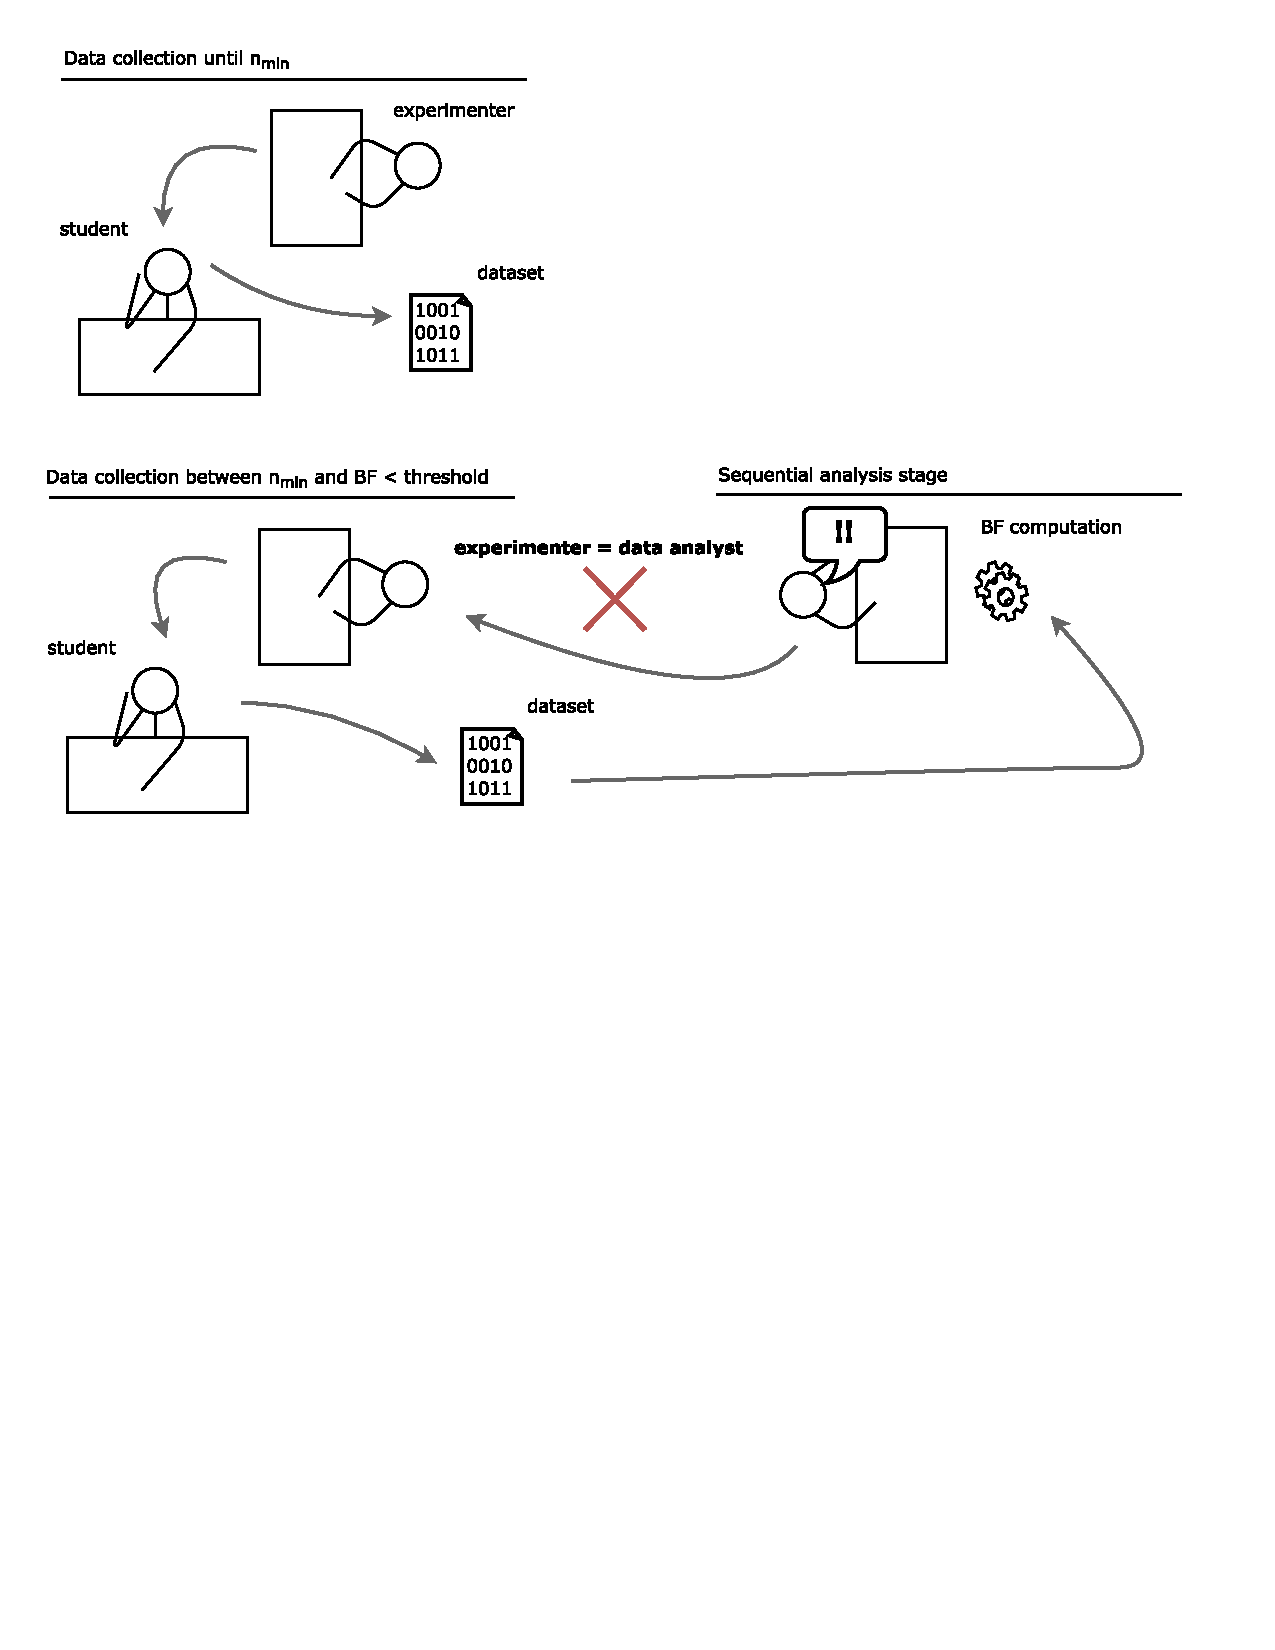
\includegraphics[width=0.8\textwidth]{figures/bias_diag.pdf}
  \label{fig:diag1}
\end{figure}

\subsubsection{Consequence 1: biased sampling, biased inference}

...parler ici de la première conséquence, i.e., le fait que l'échantillonnage soit biaisé: on atteindra plus vite / lentement le seuil pré-défini...

\subsubsection{Consequence 2: inadequacy of statistical tests, non-independance of errors...}

...parler ici de la conséquence 2, i.e., le fait que le biais de l'expérimentateur introduit une dépendance (une corrélation) entre les observations, et donc rend caduque la plupart des tests statistiques...this kind of correlated data would be thus better modeled by a time series analysis...

\subsection{Solutions ? Blind yourself.}

...blinding (double or triple)...

\subsubsection{Solution 1: one analyst, one experimenter}

...blah blah...

\subsubsection{Solution 2: one analyst-experimenter, "software-blinded"}

...this solution is relatively costless. To demonstrate this, we added a very short append to the \texttt{seqBF} function, written by Félix Schönbrodt \& Richard Morey (available \href{https://raw.githubusercontent.com/richarddmorey/BayesFactorExtras/master/BayesFactorExtras/R/seqBF.R}{here}), so that the user can now simply set the \texttt{blind} argument to \texttt{TRUE} and thus be completely blind to the results of the sequential BF computations. The only output is a sentence that either indicates to "continue" or to "stop" the recruitment, considering the threshold pre-defined by the user (see \nameref{sec:supp} for code details).

\section{What does look like SEAB ?}

...the SEAB can wear several forms as we expect different kind of behaviors of the SBF design according to the researcher's "a priori" expectancies and the effect size. Moreover, we focus here on the simplest case in which the expectancies of the researcher are constant throughout the sequential testing. Although non realistic, this setting serves illustrative purposes in the next section.

\subsection{Predictions}

...présenter ici nos prédictions, i.e., ce qu'on s'attend à observer sur l'évolution du SBF dans deux cas (H0 et H1 taille d'effet moyenne, par exemple), selon un chercheur avec des a priori différents...la Figure \ref{fig:pred} illustre nos prédictions pour différents scénarios (e.g., l'expé voit une évolution de BF conforme à ses attentes, non-conforme, etc.)...created with https://www.draw.io/ ...

\begin{figure}[H]
  \caption{Predicted consequences of the SEAB on the results of a SBF procedure, for a given Cohen's d of 0.6 (hereafter, "H1") or of 0 (hereafter "H0"), according to the \emph{a priori} researcher's beliefs.}
  \centering
  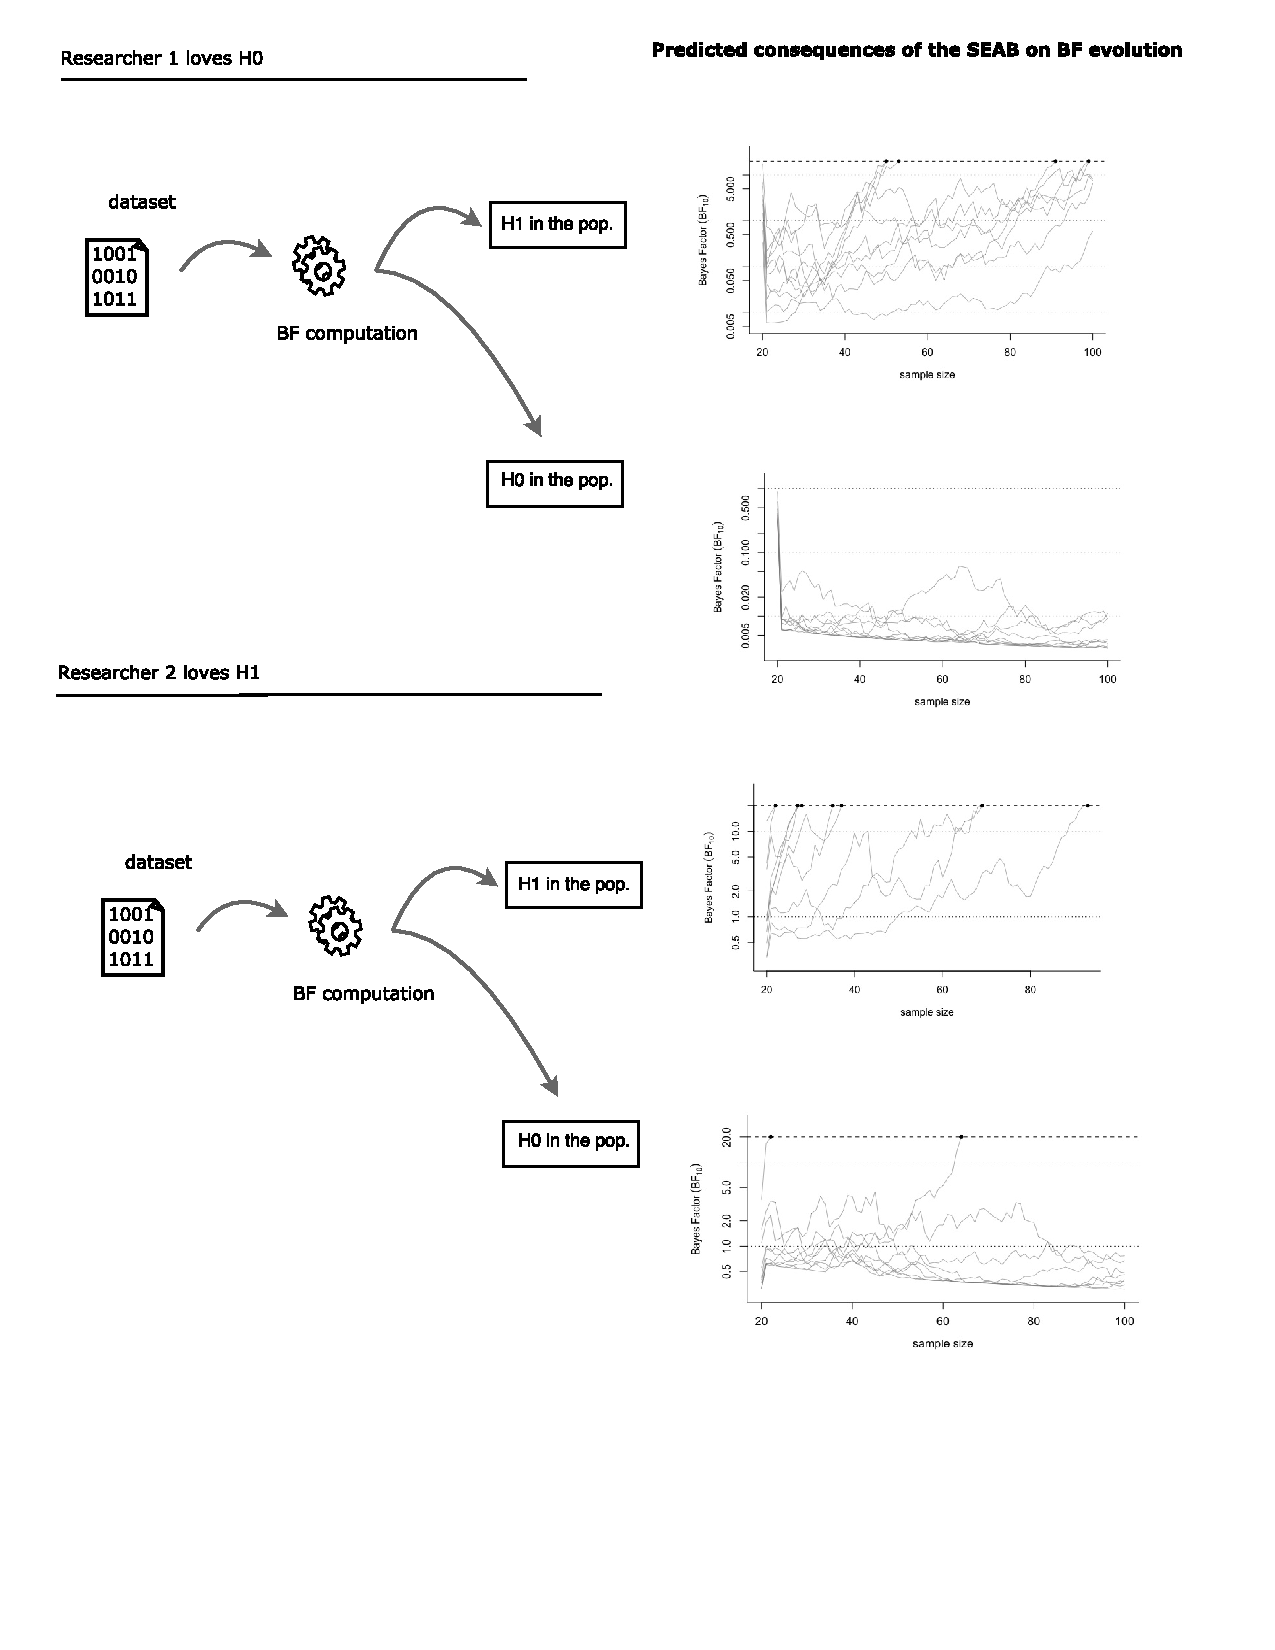
\includegraphics[width=0.8\textwidth]{figures/BFF_predictions.pdf}
  \label{fig:pred}
\end{figure}

\lnnote{peut-être ajouter un plot de l'évolution "normale" du BF pour la même taille d'effet ?}

\subsection{Experimental demonstration}

...proposer ici un protocole expérimental qui permettrait de mettre en évidence le SEAB...

\section{Conclusions}

...exemple de manip utilisant le SBF: \cite{martin_perceiving_2016}...

\section{Supplementary materials}\label{sec:supp}

...\url{https://github.com/lnalborczyk/Blind_BF}...le repo est privé pour le moment donc on ne peut pas y accéder avec ce lien, mais la fonction est dispo sur le repo Overleaf...

\section{Acknowledgements}

...many thanks to my mom...

\bibliography{BBF}

\end{document}
